%In the last years, 2D materials with interesting properties were synthesized. One of it is hexagonal boron nitride. It is made up of the same number of nitrogen and boron atoms. They are arranged in an $\textnormal{sp}^2$-bonded honeycomb lattice so that each nitrogen is neighbored by boron atoms and vice versa. The ionic bond character between both is a direct result from the nitrogens larger electrochemical negativity, withdrawing electrons from the boron lattice site and making \textit{h}-BN an insulator with wide band 

In the last years, a new family of 2D materials arose. Its most known member, graphene, already attracted much attention in the research community. Graphene, a $\textnormal{sp}^2$-bonded carbon honeycomb lattice, has shown remarkable electronic and mechanic features determined by the atomic type and bond configuration. With careful preparation methods, large layers of defect free graphene are grown on a variety of substrates. Within this layer, a linear band dispersion is formed at the corners of the Brillouin zone (Dirac cones), that promote high charge carrier mobilities (cite).

Hexagonal boron nitride (\textit{h}-BN) is isostructural and -electronical to graphene, but every second lattice site is occupied by nitrogen, every other by boron. The nitrogens larger electrochemical negativity - withdrawing electrons from the boron side - results in an ionic bond character between B \& N. Compared to the covalent bond formation in graphene that facilitates its conductivity, the ionic bond character makes \textit{h}-BN a wide band gap ($\approx \SI{6}{\eV}$) insulator. \cite{watanabe_direct-bandgap_2004, cassabois_hexagonal_2016, blase_quasiparticle_1995} 

Free standing \textit{h}-BN is investigated with \textit{ab-initio} calculations \cite{han_effects_2014,mortazavi_investigation_2012,topsakal_first-principles_2009,peng_mechanical_2012}. Together with experiments \cite{paszkowicz_lattice_2002} a RT crystal lattice constant of $a_{\textit{h}-BN, RT}=\SI{2.504}{\angstrom}$ is derived.  It can be grown on a variety of metal surfaces.\cite{muller_epitaxial_2010,muller_one-dimensional_2008,guo_controllable_2012-4,siegel_heterogeneous_2017,schwarz_corrugation_2017,joshi_boron_2012,preobrajenski_monolayer_2005,vinogradov_one-dimensional_2012,farwick_zum_hagen_structure_2016,schulz_epitaxial_2014,Schulz_Templated_2013,gomez_diaz_hexagonal_2013,usachov_experimental_2012,orlando_epitaxial_2012,preobrajenski_monolayer_2007-1,preobrajenski_monolayer_2005,auwarter_synthesis_2004-1,auwarter_xpd_1999,nagashima_electronic_1995,corso_h-bn_2005,morscher_formation_2006,nagashima_electronic_1995,cavar_single_2008,muller_symmetry_2005,nagashima_electronic_1995,gomez_diaz_hexagonal_2013,dong_how_2010,brugger_reversible_2010,preobrajenski_monolayer_2007-1,berner_boron_2007,corso_boron_2004,brugger_comparison_2009,goriachko_self-assembly_2007}


 Depending on the substrates used, different lattice mismatches can be achieved. Many geometric corrugations can be achieved with increasing lattice mismatch and substrate-\textit{h}-BN interaction. Since this interaction is believed to have its origin in the partially filled d-states of the substrate,\textcolor{red}{\textbf{citation}} transition metal substrates are widely used. While substrates exist where the lattice constant are virtually identical (Ni: $\Delta \leq \SI{0.5}{\percent}$), other substrates show large mismatches (Ag(111): $\Delta \approx \SI{14}{\percent}$).

The growth of \textit{h}-BN on nearly lattice matched Ni(111) resulted in uniform commensurate layers. With increasing lattice mismatch, moir\'e patterns are formed on Pd and Pt. The stronger interaction of \textit{h}-BN and Rh(111) results in a corrugated nanomesh to be formed on the substrate.\textcolor{red}{\textbf{citation}} Even 1D structures are reported on Fe(110) \cite{vinogradov_one-dimensional_2012} and Cr(110) \cite{muller_one-dimensional_2008}. 

Here we consider \textit{h}-BN on Cu(111) ($\Delta \approx \SI{2}{\percent}$) as example system of self-limited growth and highlight most relevant insights reported in literature.\cite{joshi_boron_2012, schwarz_corrugation_2017, auwarter_hexagonal_2018}

\subsubsection{\textit{h}-BN on Cu(111)}
%\begin{table}\centering
%	\caption{Lattice mismatches between \textit{h}-BN and several transition metal surfaces. The mismatch is given to describe the relative size of the \textit{h}-BN layer compared to the substrate, e.g. negative values indicate a larger lattice constant in the substrate bulk. Information adopted from \cite{_ptable}}
%	
%	\begin{tabular}{cccl}
%		Substrate 	& Mismatch [\%] 		& Electronic configuration \\ \hline
%		Ni(111)		& \SI{+0.4}{\percent} 	& [Ar] 3d8 4s2	\\
%		Cu(\left( 111)		& \SI{-1.9}{\percent} 	& [Ar] 3d10 4s1	\\	
%		 \\
%	\end{tabular}
%	\label{tab:h-BN-mismatch}
%\end{table}

	\paragraph{Stoichiometry}
	XPS measurements (see \autoref{fig:XPS-hbn-Cu111-martin}) show B\textit{1s} and N\textit{1s} components in a 1:1 ratio, indicating that the layer retains the precursor stoichiometry during growth, but all hydrogens are cleaved from the precursor prior to layer formation and desorp from the sample.\cite{Zhang_Two-dimensional_2017}
	
\begin{figure} \centering
	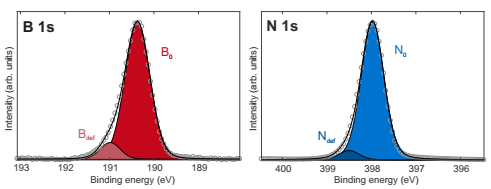
\includegraphics[width=0.7\textwidth]{./images/XPS-hbn-Cu111-martin}%
	\caption{XPS of a full ML \textit{h}-BN on Cu(111) grown with CVD of borazine. Fit components $B_0$ ($E_b=\SI{190.4}{\eV}$), $N_0$ ($E_b=\SI{398.0}{\eV}$) and $B_{def}$ ($E_b=\SI{191.0}{\eV}$) and $N_{def}$ ($E_b=\SI{398.5}{\eV}$) are assigned to pristine \textit{h}-BN layer and defective components respectively. Adopted from \cite{schwarz_assembly_2018}}
	\label{fig:XPS-hbn-Cu111-martin}
\end{figure}

	\paragraph{Moir\'e geometry}
	The properties of various moir\'e superstructures are well described in literature and Hermann gives a comprehensive overview in his paper.\cite{hermann_periodic_2012}\label{section:moire}
	A moir\'e is always present if an over layer shows a lattice mismatch with respect to the substrate. 
	Here the two most important examples are given, i.e. for an overlayer with the substrate Bravais lattice (hexagonal) either aligned with the substrate basis or rotated by an angle $\alpha$.
	
	For \textbf{isotropically scaled and aligned over layers} one can calculate the scaling factor $$p=\frac{R^{'}_{O1}}{R_{O1}}$$ which gives the size of the over layer lattice $R^{'}_{O1}$ in units of the substrate lattice $R_{O1}$. The moir\'e pattern shows the same bravais lattice type than the substrate\cite[10]{hermann_periodic_2012}. If moir\'e and ad layer lattice are aligned ($\alpha=0$\textdegree) the direction of moir\'e and substrate is aligned. The period of the moir\'e calculates to $$a_{moir\'e}=\underbrace{\frac{p}{|p-1|}}_{\kappa}a_{substrate}$$
	With $a_{moir\'e}$ and $a_{substrate}$ are experimentally available, the ad layer lattice can be calculated with high precision (usually one order of magnitude more accurate than direct measurement of its period).\cite{farwick_zum_hagen_structure_2016}

Depending on the relative orientation of \textit{h}-BN and substrate the moir\'e period changes. Although large domains with uniform orientation can be grown on single crystal substrates (\autoref{fig:moire-STM-model}(a,c)), rotational domains exist(\autoref{fig:moire-STM-model}(b,d,e)).
The model representation nicely shows the change in moir\'e period when
\autoref{fig:moire-STM-model}(c) shows a case where the \textit{h}-BN ad layer has the same unit cell orientation than the copper. For a \textbf{isotropically scaled and rotated over layer} the angle between substrate and moir\'e ($\gamma$[rad]) scales with the angle between over layer and substrate ($\alpha$[rad]) as $\alpha=(1-p)\gamma$.
In this case, one can determine $\alpha$ and $p$ from experimental observables $\gamma$(moir\'e angle to substrate) and $\kappa$(scaling factor) through relations $$ \alpha=\arctan \left ( \frac{sin(\gamma)}{cos(\gamma)+\kappa} \right )\qquad p=\frac{\kappa}{\sqrt{1+\kappa^2+2\kappa cos(\gamma)}}$$

\begin{figure} \centering
	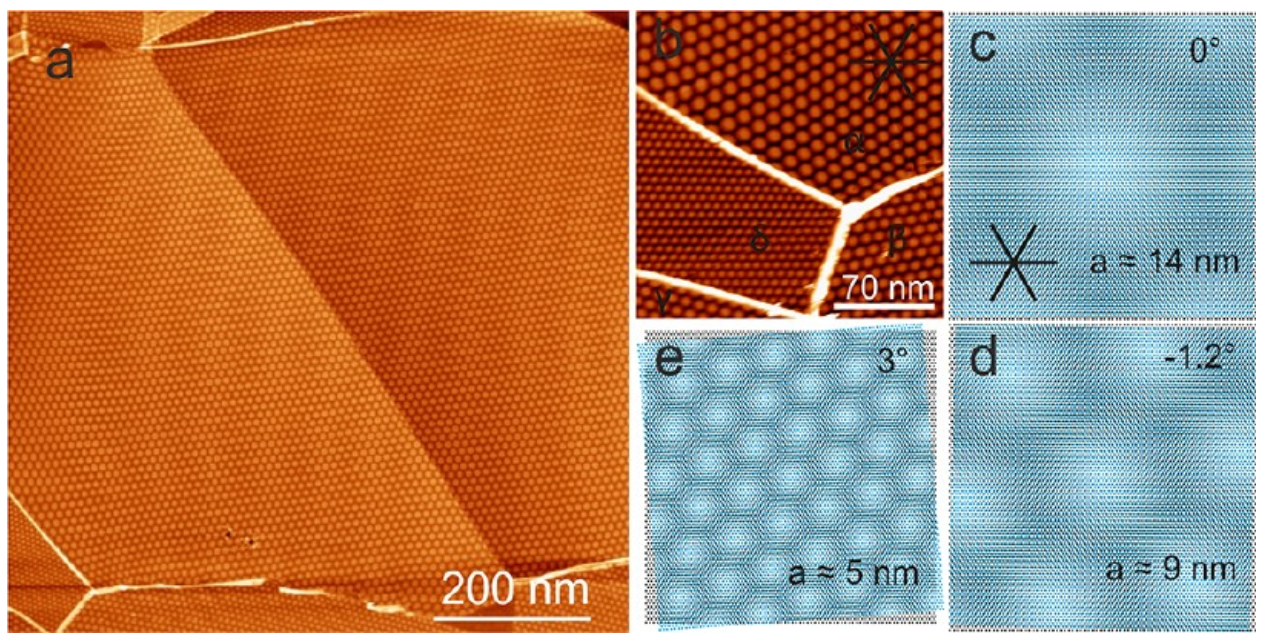
\includegraphics[width=0.9\textwidth]{./images/h-BN-cvd-cu111.png}%
\caption{(a) STM topography of \textit{h}-BN on Cu(111). Large domains with uniform orientation and moir\'e period are formed after CVD growth. (b) Different rotational domains are observed that show different moir\'e periods, reproduced by three models (c-e) where different \textit{h}-BN rotations are shown together with the resulting moir\'e periods a. Adopted from \cite{joshi_boron_2012}}
\label{fig:moire-STM-model}
\end{figure}

As mentioned above the orientation of the moir\'e superstructure is determined by the relative ad layer rotation alone, while its period is determined by lattice mismatch, too. This results in a variety of moir\'e superstructure orientations and periods, strongly related to the used substrate.
	
\paragraph{Periodic change in work function}
A direct result of the lattice mismatch between \textit{h}-BN and Cu(111) is the changing registry of ad layer atoms and substrate. The periodic modulation of B/N registry to the substrate atoms results in regions of stronger and weaker interaction between \textit{h}-BN and substrate and is the reason for the nano templating effect of \textit{h}-BN on many substrates.\textcolor{red}{\textbf{citation}} In the following some effects are discussed that lay the foundation for a nano patterning effect of \textit{h}-BN and its influence on the electronic structure of adsorbates.

While a first report in 2004 \cite{corso_boron_2004}, pointed to the formation of a complicated two layer structure, later experiments \cite{roth_chemical_2013, li_grain_2015} including ours \cite{joshi_boron_2012, schwarz_corrugation_2017} proofed a single layer of B \& N atoms in a regular hexagonal lattice when grown on Cu(111). It evolved as well investigated system to perform experiments on. After CVD growth it adsorbs on Cu(111) as a flat layer. Due to its  lattice mismatch, "hill" regions  (corresponding to a $N_{top}B_{fcc}$ registry) and "valley" regions (corresponding to a $N_{fcc}B_{hcp}$ registry) are formed. In these regions the work function is altered in opposite directions. While larger at the hill/pore regions, the work function reduces continuously to its lowest value in the valley/wire regions.\footnote{Please note that the notation is not uniform throughout the literature. Sometimes hills are referred to as pores and valley regions are denoted as wire regions.} 

After growth of \textit{h}-BN the substrates total work function is reduced [e.g. Rh: \SIrange{5.1}{3.07}{\eV} \cite{gomez_diaz_hexagonal_2013}. Therefor a dipole moment $\mu$ pointing from the the bulk to the surface is necessary, rather likely created by a negative charge transfer from the bulk into the ad layer.\cite{roman_periodic_2013}

Everywhere two regions with different work functions meet, local electrostatic fields arise to compensate for the vacuum level misalignment.
\begin{figure} \centering
	\subfigure[Work function variation along \textit{h}-BN/Cu(111) moir\'e. (a) STM image showing the \textit{h}-BN moir\'e with a periodicity of \SI{8.4}{\nano \meter}. Scan parameter: $U_b = \SI{4.0}{\volt}, I_t = \SI{40}{\pico \ampere}$. (b)	Field emission resonances acquired along the black dotted line in a) revealing a variation of the peak positions. (c) Work  function  differences  between bright  (“hill”/pore)  and  dark  (“valley”/wire)  regions obtained  from  the  dI/dV curves  of  the  field emission  resonances  displayed  in  b). Adopted from \cite{schwarz_corrugation_2017}]{
		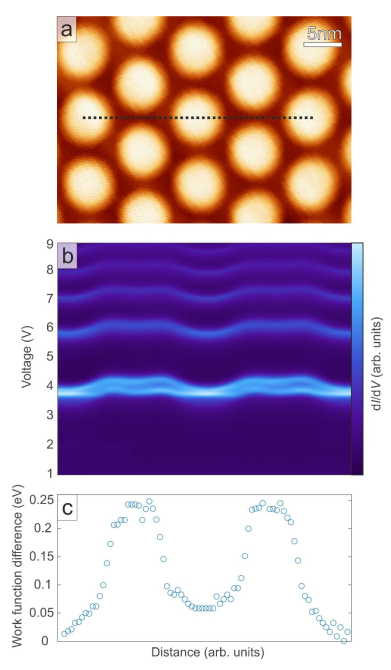
\includegraphics[width=5cm]{./images/h-BN-Cu(111)-wf-change}
	\label{fig:h-BN-Cu(111)-wf-change-I}
		} \quad
	\subfigure[Position dependent energy level alignment of $NC-Ph_4-CN$ on \textit{h}-BN/Cu(111). Three spectra are compared, recorded on molecules at valley (blue) and hill positions (green). A spectrum of the bare Ag(111) is shown as reference (yellow). STM images at different bias voltages are shown (b-g). While at low bias (b) all molecules appear in the same contrast, molecules residing at the hill positions contribute at lower bias (b-d) to the tunneling current than molecules in the valley regions where molecular orbital energies are shifted to higher energies. Increasing the bias (e-g) incorporates molecules at valley positions into the the tunneling process. Taken from \cite{diss-joshi}]{
	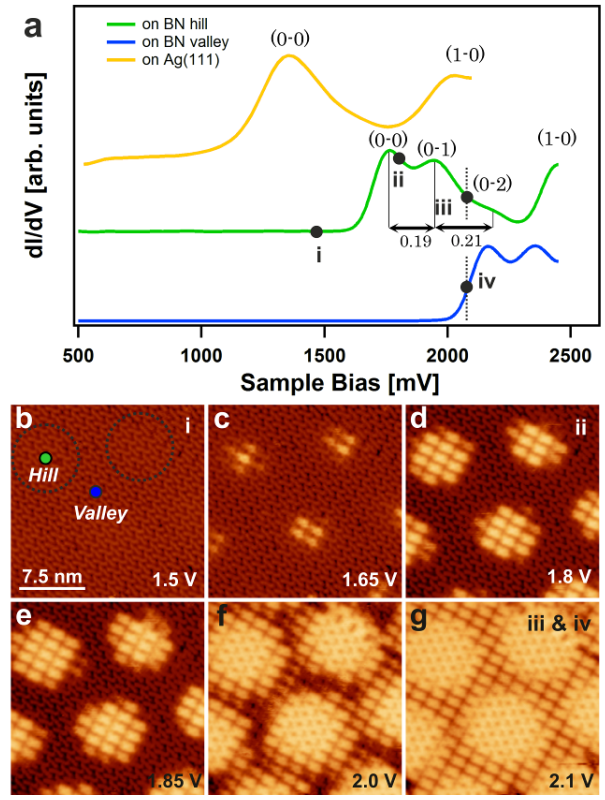
\includegraphics[width=6cm]{./images/h-BN-Cu(111)-wf-change-II}
	\label{fig:h-BN-Cu(111)-wf-change-II}
	}
	\caption{Workfunction change for pristine \textit{h}-BN/Cu(111) (\subref{fig:h-BN-Cu(111)-wf-change-I}) and for adsorbed molecules on \textit{h}-BN/Cu(111) (\subref{fig:h-BN-Cu(111)-wf-change-II}). For pristine \textit{h}-BN/Cu(111) the position depended change in workfunction is shown by a variation in the field emission resonances. \subref{fig:h-BN-Cu(111)-wf-change-II} After adsorption of molecules a shift in molecular orbital energy is emphasized by single point spectra taken at different positions within the moir\'e unit cell. This spatial variation can be visualized by STM images taken at the right bias voltages.}
	\label{fig:h-BN-Cu(111)-wf-change}
\end{figure}

\FloatBarrier
\subsection{Molecular assembly on \textit{h}-BN}
\label{section:Mol-on-h-BN}
With changing work function, a lateral electric field emerges. For gr/Ru(0001) lateral dipole pointing from valley to pore sites arise.\cite{zhang_assembly_2011} It can be used to trap adsorbates with dipole moment along the field lines. This was shown for FePc and pentacene molecules on a graphene/Ru(0001) substrate. Here FePc molecules adsorp first on regions with high lateral dipole along top-fcc direction (valley), followed by regions with lower lateral dipole (on the hill). Pentacene molecules are trapped along the top-fcc direction, too.\cite{zhang_assembly_2011}  This general adsorption mechanism is applicable for other systems with periodic modulation of the work function.

\autoref{fig:h-BN-Cu(111)-wf-change} depicts the work function change measured with STS (Field emission resonances) indicating a similar modulation of the work function. In this theses TBP molecules (\autoref{section:TBP}) and helicene molecules (\autoref{section:helicene}) are used as sample molecules for specific adsorption site or orientation alignment.

It was shown that this moir\'e superstructure influences molecular assembly. 
\textcolor{red}{\textbf{Explain the Porphine adsorption on metal and on \textit{h}-BN}}

\begin{figure} \centering
	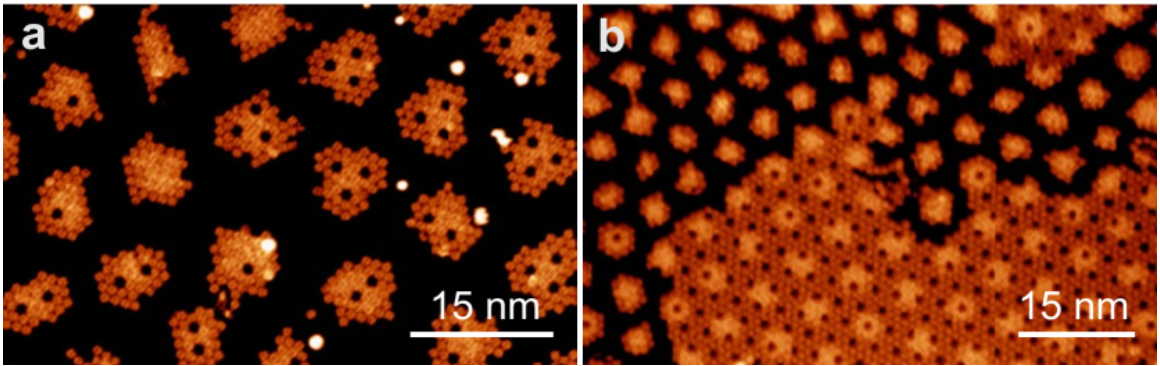
\includegraphics[width=0.7\textwidth]{./images/2H-P-hBN-Cu111-joshi}%
	\caption{STM topography of 2H-P adsorped on \textit{h}-BN/Cu(111). (a) A large moir\'e domain guides the formation of small 2H-P islands with off center vacancies. (b) High coverage overcomes the template effect of the \textit{h}-BN support. Adopted from \cite{diss-joshi}}
	\label{fig:2H-P-hBN-Cu111-joshi}
\end{figure}

\textbf{Molecules are electronically decoupled} when adsorped on a \textit{h}-BN spacer layer on top of a metal. The insulating \textit{h}-BN hinders the metal to influence molecular properties by charge transfer, image potentials etc.\textcolor{red}{\textbf{citation}}. As a result, molecular orbitals are unperturbed and can be imaged in STM/STS.